\section{Smart/Intelligent Windows}
%Smart windows (or intelligent windows) are defined as a type of window that partially blocks the
%solar radiation in hot weather and transmitts the solar radiation in cold weather by changing its
%thermal and radiative properties (dynamically) (\cite{Kamalisarvestani2013}:(25)). 
Smart windows (or intelligent windows) is a type of windows that manages to 
regulate the transmitted solar radiation by changing its optical properties.
The change in its optical properties can be
obtained by adding a controllable absorbing layer on the surface of the glass. 
The ability of the smart window to optimize solar flux and daylight may help to
reduce the electricity loads regarding heating, cooling and lighting.
%The use of smart windows may help to reduce heating, cooling and electricity loads in buildings.
They should optimally also be able to adapt to the difference created by the seasons. E.g. summertimes
have a different demand than wintertimes with respect to the thermal properties of the window.
%\cite{Dussault2012} \cite{Jelle2010} \cite{white1999}
\cite{Dussault2012,Jelle2010,White1999}
Windows with such a
switchable layer can be categorized into two systems: active and passive. The active switchable glazing 
systems require an external triggering mechanism and offers supplementary options compared to 
passive systems. An example of this is the electrochromic window. 
However, their dependency on a power supply and additional 
electronical curcuits makes them not as attractive as their passive counterparts.  
The passive devices do not require an external energy source, but switches automatically
subject to environmental change. Examples of such devices are: photochromic windows reacting to 
light and thermochromic windows, which change in accordance to the temperature 
(\cite{Kamalisarvestani2013}:\cite{Baetens2010}).
%
\begin{figure}[h!]
  \centering
   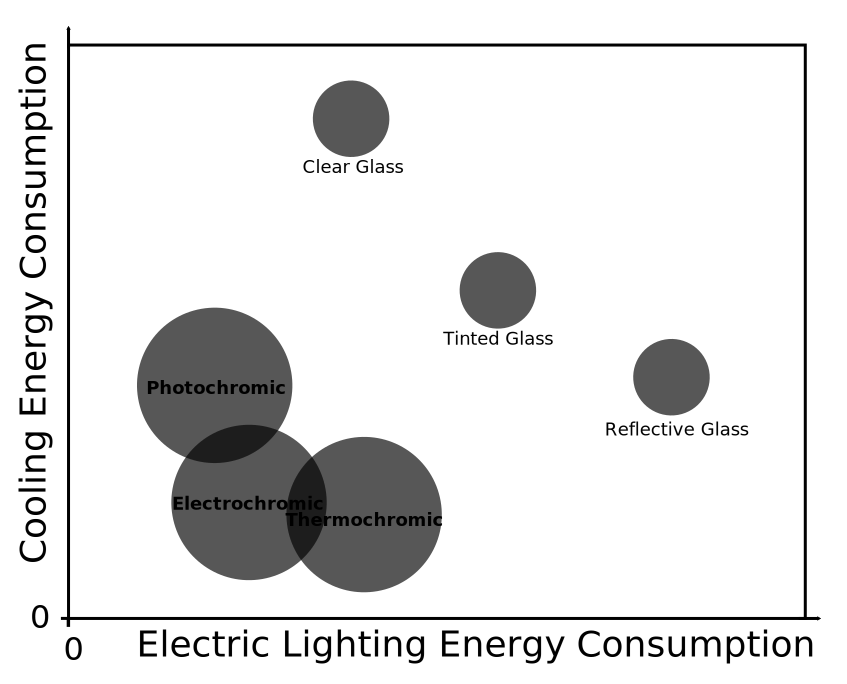
\includegraphics[width=0.5\textwidth]{Figures/chromicGlassComparison.pdf}
   \caption{Comparison of the electric lighting energy and cooling energy consumption between different
   glazing types. Adapted from (\cite{Huovila2007},p.20). 
   }
   \label{fig:energyComparison}
\end{figure}
%
As shown in Figure \ref{fig:energyComparison} the resulting energy load varies for the different
window and glazing technologies. 
It also demonstrates an important fact: even though using reflective glass would reduce
cooling loads, a window should also be able to let visible light through! If the transmission of
the visible spectrum is to low, it could cause the need for additional lighting, which again
would increase the overall energy load (\cite{Kamalisarvestani2013},12).
%\textbf{EXTRA:} Due to lighting, a window should be able to let through visible light (\cite{Kamalisarvestani2013},12).
Electrochromic and thermochromic windows usually
result in lower cooling loads. In addition the electrochromic technology requires 
less energy for lighting. However, as argued in the review of Kamalisarvestani et al.
\cite{Kamalisarvestani2013}, the necessity of wiring for electrochromic windows and
the fact that the drawback regarding visible transmission in thermochromic windows can be
solved by appropriate doping \cite[p.~39]{Kanu2010}(70), ensures the position of 
thermochromic windows as a good and actual low-priced alternative \cite{Mlyuka2009}
\textbf{<-fikk ikke tilgang,prøv VPN}.







\section{Thermochromic Materials}
%Materials that change their optical nature when subject to irradiation by light(photons),
%temperature change or an applied electric field are called photochromic, thermochromic and 
%electrochromic, respectively, and are collectively called chromic materials.
%(\cite{Kiri2010},1)
%\\
%\\
%The word thermochromic originates from Greek, meaning warm or hot (''Thermos'') and color (''Chroma'').
%As mentioned earlier, thermochromic materials their optical properties in response to changes in
%temperature and results in the material changing color (\cite{Kamalisarvestani2013},74,75). 
%
The technology behind intelligent windows and its diversity, is based on
materials that change their optical properties when subject to some external physical process.
These materials are called chromic materials. 
The word chromic originates from the greek word ''Chroma'', which means color.
If the induced change of optical properties results in changing the spectral reflectance in
the visible spectrum, the material will change its color. 
\textit{?CAN I SAY THIS WITHOUT A REFERENCE? ISN*T IT PRETTY OBVIOUS FROM ALL THE OTHER INFORMATION/
TAKEN FOR GRANTED? IT IS CORRECT RIGHT??} 
Chromic materials are again subdivided into categories dependent on what triggers their optical change, 
many of which have already been mentioned.
For example, photochromic and eletrochromic materials are two categories of chromic materials 
that changes their optical properties when subject to irradiation by light (photons) or an applied 
electric field, respectively. However, another subcategory is thermochromic materials and will be the
category of interest in this assignment.
(\cite{Kiri2010},1)
%''Thermos'' is the greek word for warm or hot and thermochromic materials change their optical
%properties (like color) in response to temperature changes
%(\cite{Kamalisarvestani2013},74,75). 
The word thermochromic, compared to the ''parent'' material class, includes the extra word ''Thermos'', 
which is the greek word for warm or hot. 
As the name suggests, thermochromic materials change their optical
properties (like color) in response to heat or, in other words, the change in temperature.
%Thermochromic materials change their optical
%properties (like color) in response to temperature changes
(\cite{Kamalisarvestani2013}:(74)<-ikke tilgang(prøv VPN),\cite{Parkin2006}). 
\cite{White1999}
\\
\\
Typically, this change in color happens gradually over a range of temperatures. In this case it is called
continuous thermochromism. Discontinuous thermochromism also occurs and involves a structural
phase change at a certain characteristic ''transition temperature'' $T_t$. This phase
change can be of first or second-order in nature, and may be reversible or irreversible (\cite{Kiri2010}:(1)). 
\\
Compounds like inorganic oxides, liquid cryctals (\cite{Kiri2010}:(2)), 
conjugated oligomers (\cite{Kiri2010}:(3)), leuco dyes (\cite{Kiri2010}:(4)) can exhibit thermochromic 
color changes reversibly. Thermochromic dyes however are usually based on organic 
compounds and show color changes on heating which are not reversible.
\\
\\
To explain the process behind the chromic behaviour, assume that the thermochromic material is initially 
in its cold state called the monoclinic state . 
Here it behaves as a semiconductor, being less reflective especially in the near-infrared(IR) region. 
Heating the material to a certain temperature, known as the transition temperature 
(as mentioned earlier), will make it change from the monoclinic state to a 
rutile state. In the rutile state (hot state) the material acts like a semi-metal, reflecting 
a wide range of solar radiation. This change of state is called metal-to-semiconductor
transition (MST) \cite[p.~4565]{Blackman2009} and is fully reversible, 
co-occured with large variations in both electrical and optical properties in the near-IR range 
\cite{Morin1959}. 
\textbf{??? -> check if understood and 
correctly written. E.g. what is co-occured?} 

Because of these interesting properties, thermochromic materials have become increasingly important,
espacially through the use as ''smart coatings'' (for e.g. windows) as mentioned earlier.
Some potential thin film candidates or smart windows include substances such as
Fe$_3$O$_4$, FeSi$_4$, NbO$_2$, NiS, TiO$_2$ and VO$_2$. \cite{White1999}.
%\\
%\\
%(Main articles from section was based on \cite{Kamalisarvestani2013} and \cite{Kiri2010})\\







\section{Thermochromic Windows}
A thermochromic window, which has been meantioned serveral times earlier, is a window
with a thermochromic glazing, allowing the window as a whole to adopt the 
optical properties of the thermochromic material. Figure \ref{fig:TCcoating} is a pictorial representation
of the influence of the thermochromic coating on the window. 
%
\begin{figure}[h!]
  \centering
   \includegraphics[width=0.9\textwidth]{Figures/TCcoating2.pdf}
   \caption{Schematic representation of thermochromic materials applied as an 
   intelligent window coating \cite{Kiria2010}.
   }
   \label{fig:TCcoating}
\end{figure}
%
%Assuming that the transition temperature will $T_t$ of the material is set to the 
%thermal comfort temperature, then any temperature $T$ such that $T>T_t$ will 
Below the transition temperature $T<T_t$, the window should transmit the solar thermal radiation, heating 
up the interior of the building. If the temperature increases above the transition temperature $T_t$,
the transmission of the thermal radiation should decrease significantly, lowering or removing
the necessity of using cooling devices. For this to work, the transition temperature, which
is usually much higher than room temperature, needs to be reduced down to a thermally comfortable 
level. This can be done by adding small quantities of a foreign material into the thermochromic 
material, a process called doping.
\\
\\
%
\begin{figure}[h!]
  \centering
   \includegraphics[width=0.5\textwidth]{Figures/TCWtransmittanceMcCluney1996andKamali2013.pdf}
   \caption{The spectral transmittance of a perfect thermochromic window, shown for both 
   cold and hot environments (the monoclinic and rutile state, repsectively). 
   Adopted from \cite[p.~15]{McCluney1996} %\cite{Kamalisarvestani2013}
   }
   \label{fig:idealTCW}
\end{figure}
The ideal spectral modulation of the thermochromic coating is given in Figure \ref{fig:idealTCW} and
shows how the cold state should transmitt the majority of the solar radiation, here modeled
as a black body spectrum. In addition it shows how the hot state should reflect as much 
of the infrared and solar radiation as possible without compromising the transmission of the 
visible spectrum. As mentioned earlier, if the transmission of daylight is poor, it would 
lead to an increase of the electrical load due to the accompanying additional lighting.
\cite{McCluney1996}
%
As discussed by Blackman \cite{Blackman2009},
the optical transmission of the film is depending on the thickness of the film. Control of the film
thickness is crucial. Excessive coating thicknesses may lead to too much blocking of the visual light,
leaving the coating unsuitable for architectural application.
%
%
\begin{table}[htbp]
   \caption{The ideal optical performance of thermochromic windows (taken from \cite{Kamalisarvestani2013})
   which adapted it from \cite{Saeli2010}}
\centering
%\begin{tabular}{|c|c|c|c|p{1cm}p{1cm}p{1cm}p{1cm}p{1cm}p{1cm}p{1cm}|}
\begin{tabular}{ l l l l l}
\hline
\textbf{State}  &  \multicolumn{2}{l}{\textbf{Monoclinic/cold ($T<T_t$)}}  &  \multicolumn{2}{l}{\textbf{Rutile/hot ($T>T_t$)}} \\
\hline
Wavelength      &  Visible(\%)    &  NIR (\%)      &  Visible(\%)    &  NIR (\%) \\
Transmittance(T)&  60-65          &  80            &  60-65          &  15       \\
Reflectance(R)  &  17             &  12            &  17             &  77       \\
\hline
\end{tabular}
\label{tab:idealTCW}
\end{table}
%
In fact, for the transmission of visible light to be acceptable it should be higher than 60\%.
%Does this information come from the source of the table of from source ((93,94) Kamalisarvestani)??
The ideal performance of a thermochromic window is shown in Table \ref{idealTCW}, showing 
that the modulation of visible should be the same for the monoclinic and rutile state and 
letting in more than 60\% of the visible light.



\section{Vanadium dioxide}
\subsection{Doping of vanadium dioxide using tungsten}







%\cite{White1999}\\ 
%p.1201: sitat: ''Materials that undergo temperature-induced color changes are termed ''thermochromic''.
%The origins of thermochromism range from phase transitions in a compound (e.g. in an organic chromosphore)
%, to changes in ligand geometry or the number of solvent molecules in the coordination sphere (
%e.g. in a pure transition metal complex that derives its color from crystal field effects) (1-5).''\\
%p.1204: sitat: ''Thermochromic compounds have become increasingly important
%in recent yyear in the study and production of ''smart coatings'', that is, coatings that respond to their 
%environment. As in any thermochromic material, there is a change in color with a change in temperature. 
%Incorporated into a window system, a thermochromic material could be used to control the flux of 
%solar energy by changing the transmission of visible light in response to the heating effect of 
%sunlight. Thin films of materials sch as Fe$_3$O$_4$, FeSi$_4$, NbO$_2$, NiS, TiO$_2$ and VO$_2$ 
%could be used to control the infrared emittance and the solar transmittance of a glaze, owing to 
%their change at a threshold temperature from a semiconducting state to a metallic state (also known
%as the Mott transition temperature) \cite{Lampert1992}''
%\\
%\\
%\cite{Blackman2009}\\
%p.4565\\
%''It was found that incorporation of tungsten into the films led to an improvement in the colour from yellow/brown to green/blue depending on the level of tungsten incorporation. The films were optimized for optical transmission, thermochromic switching temperature, magnitude of the switching behaviour and colour to producefilms that are suitable for use as an energy saving environmental glass product. ''\\
%''Vanadium dioxide is a thermochromic material that is known to exist in four polymorphic forms; monoclinic VO2(M) and rutile VO2 (R) and two metastable forms VO2(A) and VO2(B)[2]. The monoclinic VO2(M) converts to rutile VO2(R) at 68 °C[3]. This is a fully reversible metal to semiconductor phase transition (MST) and is associated with large changes in electrical conductivity and optical properties in the near-IR region [4]. Above 68 °C, VO2 behaves as a semi-metal and is reflecting to a wide range of solar wavelengths whilst below the MST it behaves as a semiconductor, and reflects significantly less in the near infrared.'' \\
%''These tech-nology advances were not transferable into commercially relevant pro-ducts because of inappropriate transition temperatures, low visible light transmission, unattractive visible colours and limitedfilm durability.''\\
%p.4566\\
%''Tungsten has been shown to be the most effective dopant ion in reducing the MSTof VO2, it can optimally lower theTcto about 25 °C at 2 atom\% loading.''\\
%\\
%\\
%p.4569\\
%''Films suitable for use in architectural glazing would maximise the functional properties of the 
%coating whilst having a high transmission at 570 nm, preferably in excess of 60\% [23].
%The thermochromic properties of VO2 thinfilms are dependent on thickness, the largest changes in 
%optical properties are seen above a critical thickness of 70 nm [14]. The ideal film would have the 
%maximum acceptable thickness which corresponds to the minimum acceptable optical transmission. In 
%our case this is in the range 70–90 nm thick. Also the film must be adherent and visually appealing.''
%p.4569\\
%direkte sitat '' Conclusion: Thin films of VO2, suitable for use in architectural glazing, have
%been deposited onto glass substrates using a reliable and reproducible APCVD method. Changing the 
%ratio of vanadium precursor to water alters the appearance of thefilms from powdery brown to 
%adherent and transparent, with an improvement to a greener colour. This change is also accompanied 
%by a change in the transmission of the films in the near infrared and the size of the MST is dependent 
%on the thickness of thefilm being above a certain level. Controllable doping of the films with tungsten
%is demonstrated. This allows the tem-perature at which the thermochromic switch occurs to be 
%controlled. A benefit of tungsten doping is the films obtain an attractive blue colour in transmission
%further improving the aesthetic properties.''
%\\
%\\
%Seems like the figures of this paper has done experiment with VO2 using 150nm,800nm and 30nm films.
%\\
%\\
%Also, blackman mentions how the earlier work with VO2 thin films lacked control of film thickness 
%which is crucial for optimizing the optical transmission. This resulted in that even though 
%they had the required switching temperature, the excessive thickness made the 
%optical transmission too low and therefore unsuitable for application in architectural glazing. 

%\cite[p.~39]{Kanu2010}
%"The most promising thermochromic
%material for window glazing is vanadium (IV) oxide, owing to its relativity low
%transition temperature of 68◦C; however, this is still not low enough for it to
%be actually used on a larger scale. The introduction of some particular dopents
%lowers the Tc to a suitable temperature". 




%\textbf{Disposition:}\\
%Requirements\\
%- Ideal behavior- RADIATION FIGURE and PICTOGRAM\\
%- ambient transition temperature\\
%- 60\% transmittance in visible range, for lighting\\
%-  *Doping\\
%-  *Stress/strain\\
%-  *thickness\\
%\\
%- price and mass producable: materials used and current technology\\
%\\
%Best Candidates:\\
%(strengths and weaknesses)\\
%-VO2 \\
%-etc...\\



(The switchable reflective device (or dynamic tintable window)) 

\begin{thebibliography}{9}

      \bibitem{McCluney1996}
      McCluney R, Center FSE. 
      Fenestration solar gain analysis. 
      Citeseer 1996.
      
      \bibitem{Kiri2010}
      Kiri P, Hyett G, Binions R.
      Solid state thermochromic materials.
      Advances Material Letters 2010;1(2):20.

      \bibitem{Huovila2007}
      Huovila P, Ala-Juusela M, Melchert L, Pouffary S. 
      Buildings and climate change: status, challanges and opportunities.
      United Nations Environment Programme 2007.

      \bibitem{Dussault2012}
      Dussault J-M, Gosselin L, Galstian T. 
      Integration of smart windows into building design for reduction of yearly overall 
      energy consumption and peak loads.
      Solar energy 2012;86(11):3405-16

      \bibitem{Jelle2010}
      Jelle BP, Gustavsen A.
      Dynamic solar radiation control in buildings by applying electrochromic materials.
      %Zero emsion buildings-proceedings of 
      Renewable Energy Conferance/Advanced materials technologies 2010; :133%-144
      \textbf{er dette riktig?}
      %lenker: 
      %file:///home/jorgevag/Downloads/Dynamic%20Solar%20Radiation%20Control%20in%20Buildings%20by.pdf
      %http://www.zeb.no/index.php/conference-papers/item/140-dynamic-solar-radiation-control-in-buildings-by-applying-electrochromic-materials
      \bibitem{Baetens2010}
      Baetens R, Jelle BP, Gustavsen A. Properties, requirements and possibilities of smart windows
      for dynamic daylight and solar energy control in buildings: a state-of-the-art review.
      Solar energy materialsand solar cells 2010;94(2):87-105.

      \bibitem{Parkin2006}
      Parkin IP, Manning TD.
      Intelligent thermochromic windows.
      Journal of Chemical Education 2006;83(3):393.
      %    journal               year; vol. (No.): page of referance

      \bibitem{White1999}
      White MA, LeBlanc M.
      Thermochromism in commercial products.
      Journal of Chemical Education 1999;76(9):1201,1204 %1201-1205
      \bibitem{Lampert1992}
      Lampert CM.
      Smart windows switch on the light.
      IEEE Circuits Devices Mag. 1992; 8(2):19 %19-26

      \bibitem{Blackman2009}
      Blackman CS, et al. 
      Atmospheric pressure chemical vapour deposition of thermochromic tungsten doped vanadium dioxide 
      thin films for use in architectural glazing. 
      Thin Solid Films 2009;517(16):4565-70.

      \bibitem{Morin1959} 
      Morin F.
      Oxides which show a metal-to-insulator transition at the Neel temperature.
      Physical Review Letters 1959;3(1):34-6

      \bibitem{Saeli2010}
      Saeli M, et al.
      Energy modelling studies of thermochromic glazing. 
      Energy and buildings 2010;42(10):1666-73.

      \bibitem{Kanu2010}
      Kanu SS, Binions R. 
      Thin films for solar control applications. 
      Proceedings of the Royal Society of London series A 2010;466(2113):19-44

      \bibitem{Mlyuka2009}
      Mlyuka N, Niklasson G, Granqvist CG. 
      Thermochromic multilayer films of VO$_2$ and TiO$_2$ with enhanced transmittance.
      Solar Energy Materials and Solar Cells 2009;93(9):1658-7
\end{thebibliography}
